\subsection{MNIST}\label{mnist}
The ``modified National Institute of Standards and Technology'' dataset comprises a collection of 70,000 handwritten digits carefully divided into a training set of 60,000 images and a test set of 10,000 images. Each digit is represented in a grayscale image of 28$\times$28 pixels, and offers a wide range of styles and shapes. This feature makes MNIST not only an ideal starting point for novices in the field of machine learning, but also a benchmark for evaluating the performance of different image classification models. Some examples of the dataset can be seeen in Figure~\ref{fig:MNIST}

\begin{figure}
    \centering
    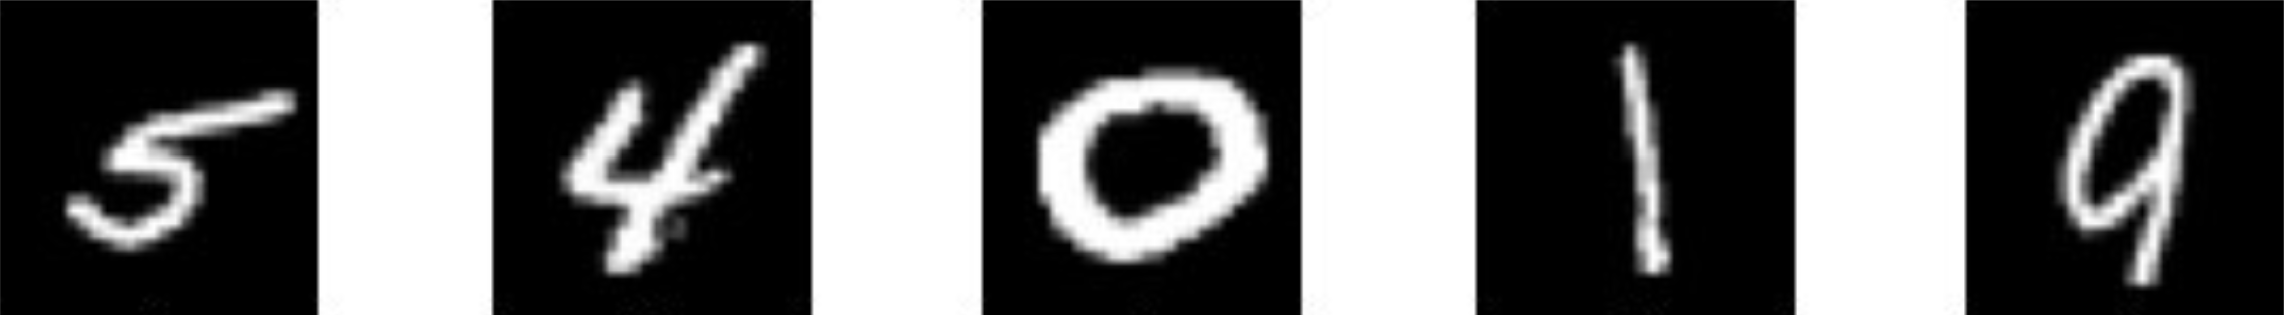
\includegraphics[width=0.3\textwidth]{figures/MNIST.png}
    \caption{Example greyscale images of the MNIST dataset - CHANGE IMAGE - RENDER OWN!!!}\label{fig:MNIST}
\end{figure}


In our project, the MNIST dataset provided a foundational experience that allowed us to understand the basics of neural network architecture and effectively implement them for the task of classifying numbers.



\subsection{MedMNIST}\label{medmnist}
//TODO